\documentclass{beamer}
\usepackage{bibentry}
\bibliographystyle{plain}

\usepackage[utf8]{inputenc}
\usepackage[T1]{fontenc}
\usepackage{lmodern}
\usepackage[frenchb]{babel}
\usepackage{graphicx}

%\usetheme{Rochester}
\setbeamertemplate{navigation symbols}{}
\setbeamertemplate{footline}[frame number]
\renewcommand{\footnoterule}{}
\newcommand{\etal}{\emph{et al.}~}

\title{%
  Comité de Suivi de Thèse \\
  {\bf Calcul de WCET par analyse de modèles temporisés}}
\author{%
  Armel Mangean \\
  {\small\tt armel.mangean@irccyn.ec-nantes.fr}}
\institute{%
  École Centrale de Nantes \\
  IRCCyN, équipe Sytème Temps-Réel}
\date{Juin 2015}

\begin{document}

  \begin{frame}
    \small
    \nobibliography{refs.bib}
    \titlepage
  \end{frame}

  \section*{Activités annexes}
  \begin{frame}
    \frametitle{\secname}

    \begin{block}{Formations doctorales}
      \begin{itemize}
        \item 17 heures de formation professionnelle
        \item 15 heures de formation scientifique
      \end{itemize}
    \end{block}

    \begin{block}{Enseignements}
      \begin{itemize}
        \item 40 heures de vacation
        \item Étudiants de DUT Informatique
        \item Cours sur les réseaux informatique
      \end{itemize}
    \end{block}
  \end{frame}

  \begin{frame}
    \frametitle{Calcul de WCET par analyse de modèles temporisés}
    \tableofcontents
  \end{frame}

  % Deux points essentiels au calcul de WCET :
  %  - un modèle des composantes logicielles
  %  - un modèle des composantes matérielles
  \section{Calcul de WCET}
  \begin{frame}
    \frametitle{\secname}

    \begin{block}{\textit{Worst Case Execution Time}}
      \begin{itemize}
        \item \og Pire cas de temps d'exécution \fg \\
          $\rightarrow$ Borne supérieure sur les temps d'exécutions
        \item Domaine d'application : tâches isolées
      \end{itemize}
    \end{block}

    % Ici :
    % "calcul" signifie "estimation" ;
    % "Analyse dynamique" signifie "via exécution" ;
    % "Analyse statique" signifie "sans exécution".
    
    \begin{block}{Calcul de WCET}
      \begin{itemize}
        \item Estimation à partir d'analyses dynamiques ou statiques
        \item Analyse conjointe des modèles logiciel et matériel du système
      \end{itemize}
    \end{block}
  \end{frame}
  
  \subsection{Par analyse statique}
  \begin{frame}
    \frametitle{\secname}
    \framesubtitle{\subsecname}

    \begin{block}{\textit{Abstract Interpretation}}
      \begin{itemize}
        \item Approximation de la sémantique des programmes
        \item Utilisation pour l'abstraction des progammes et du matériel (cache et pipeline)
      \end{itemize}
    \end{block}

    % Problème d'optimisation :
    %  On a des variables et des contraintes ;
    %  On veut maximiser (ou miniser) une fonction de coup.

    \begin{block}{\textit{Integer Linear Programming}}
      \begin{itemize}
        \item Problème d'optimisation à variables entières et contraintes linéaires
        %\item \textit{Implicit Path Enumeration Technique}
      \end{itemize}
    \end{block}
  \end{frame}

  \begin{frame}
    \frametitle{\secname}
    \framesubtitle{\subsecname}

    \begin{exampleblock}{Approches existantes}
      \tiny
      \begin{itemize}
        \item \bibentry{HF04}
        \item \bibentry{LM95}
        \item \bibentry{BCR10}
        \item \bibentry{LYG10}
      \end{itemize}
    \end{exampleblock}
  \end{frame}

  \subsection{Par vérification formelle}
  \begin{frame}
    \frametitle{\secname}
    \framesubtitle{\subsecname}

    \begin{block}{\textit{Timed Model Checking}}
      \begin{itemize}
        \item Vérification algorithmique de satisfaction d'une propriété
          temporelle par un modèle temporisé
      \end{itemize}
    \end{block}

    \begin{block}{Analyse temporelle}
      \begin{itemize}
        \item Domaine d'application : tâches non-isolées
        \item Analyse tenant compte des autres tâches, des interruptions, du
          partage des bus et cache, ...
        \item Explosion de l'espace d'état
      \end{itemize}
    \end{block}
  \end{frame}

  \begin{frame}
    \frametitle{\secname}
    \framesubtitle{\subsecname}
    \begin{exampleblock}{Approches existantes}
      \tiny
      \begin{itemize}
        \item \bibentry{DOT10}
        \item \bibentry{CB13}
      \end{itemize}
    \end{exampleblock}
  \end{frame}

  % Bibilographie sur le permier point
  \section{Modèle du logiciel}
  \subsection{Reconstruction de CFG}
  \begin{frame}
    \frametitle{\secname}
    \framesubtitle{\subsecname}

    \begin{block}{\textit{Control Flow Graph}}
      << Graphe de flot de contrôle >> \\
      $\rightarrow$ $(V,E,i)$ avec $V$ les blocs de base, $E \subset V \times V$
      les chemins du flot de contrôle et $i \in V$ le point d'entrée
    \end{block}

    \begin{block}{Reconstruction de CFG}
      \begin{itemize}
        \item À partir d'un fichier exécutable
        \item Reconstruction des blocs de base
        \item Reconstruction des chemins du flot de contrôle
      \end{itemize}
    \end{block}
  \end{frame}

  \begin{frame}
    \frametitle{\secname}
    \framesubtitle{\subsecname}

    \begin{exampleblock}{Approches existantes}
      \tiny
      \begin{itemize}
        \item \bibentry{FLP15}
        \item \bibentry{The00}
      \end{itemize}
    \end{exampleblock}
  \end{frame}

  \subsection{Réduction de CFG}
  \begin{frame}
    \frametitle{\secname}
    \framesubtitle{\subsecname}

    % Comportement équivalent vis-à-vis d'un comportement spécifié
    % Suppression des instructions non concerné : réduction du modèle
    \begin{block}{\textit{Program Slicing}}
      $\rightarrow$ Calcul de l'ensemble des instructions affectant l'état du
      programme à un point précis de son exécution
    \end{block}

    \begin{block}{Réduction de CFG}
      \begin{itemize}
        \item Suppression des instructions n'influant sur le flot de contrôle
        \item Contention de l'explosion de l'espace d'état dû aux registres
      \end{itemize}
    \end{block}
  \end{frame}

  \begin{frame}
    \frametitle{\secname}
    \framesubtitle{\subsecname}
    \begin{exampleblock}{Approches existantes}
      \tiny
      \begin{itemize}
        \item \bibentry{Wei81}
        \item \bibentry{CF97}
        \item \bibentry{KJL03}
      \end{itemize}
    \end{exampleblock}
  \end{frame}

  % Mise en oeuvre pratique sur le premier point
  \section{Développement d'un outil}
  \subsection{Conception}
  \begin{frame}
    \frametitle{\secname}
    \framesubtitle{\subsecname}
    \small
    \begin{block}{HARMLESS}
      Analyse sématique des fichiers exécutables \\
      \tiny
      \bibentry{KBB12}
    \end{block}

    \begin{block}{Haskell}
      Langage de programmation fonctionnel \\
      \tiny
      \bibentry{Mar10}
    \end{block}

    \begin{block}{Hoopl}
      Bibliothèque de manipulation de CFG \\
      \tiny
      \bibentry{RDP10}
    \end{block}

%\footnotetext{\texttt{https://github.com/LiberH/tool}}
  \end{frame}

  \begin{frame}
    \frametitle{\secname}
    %\framesubtitle{\subsecname}

    \begin{figure}
      \centering
      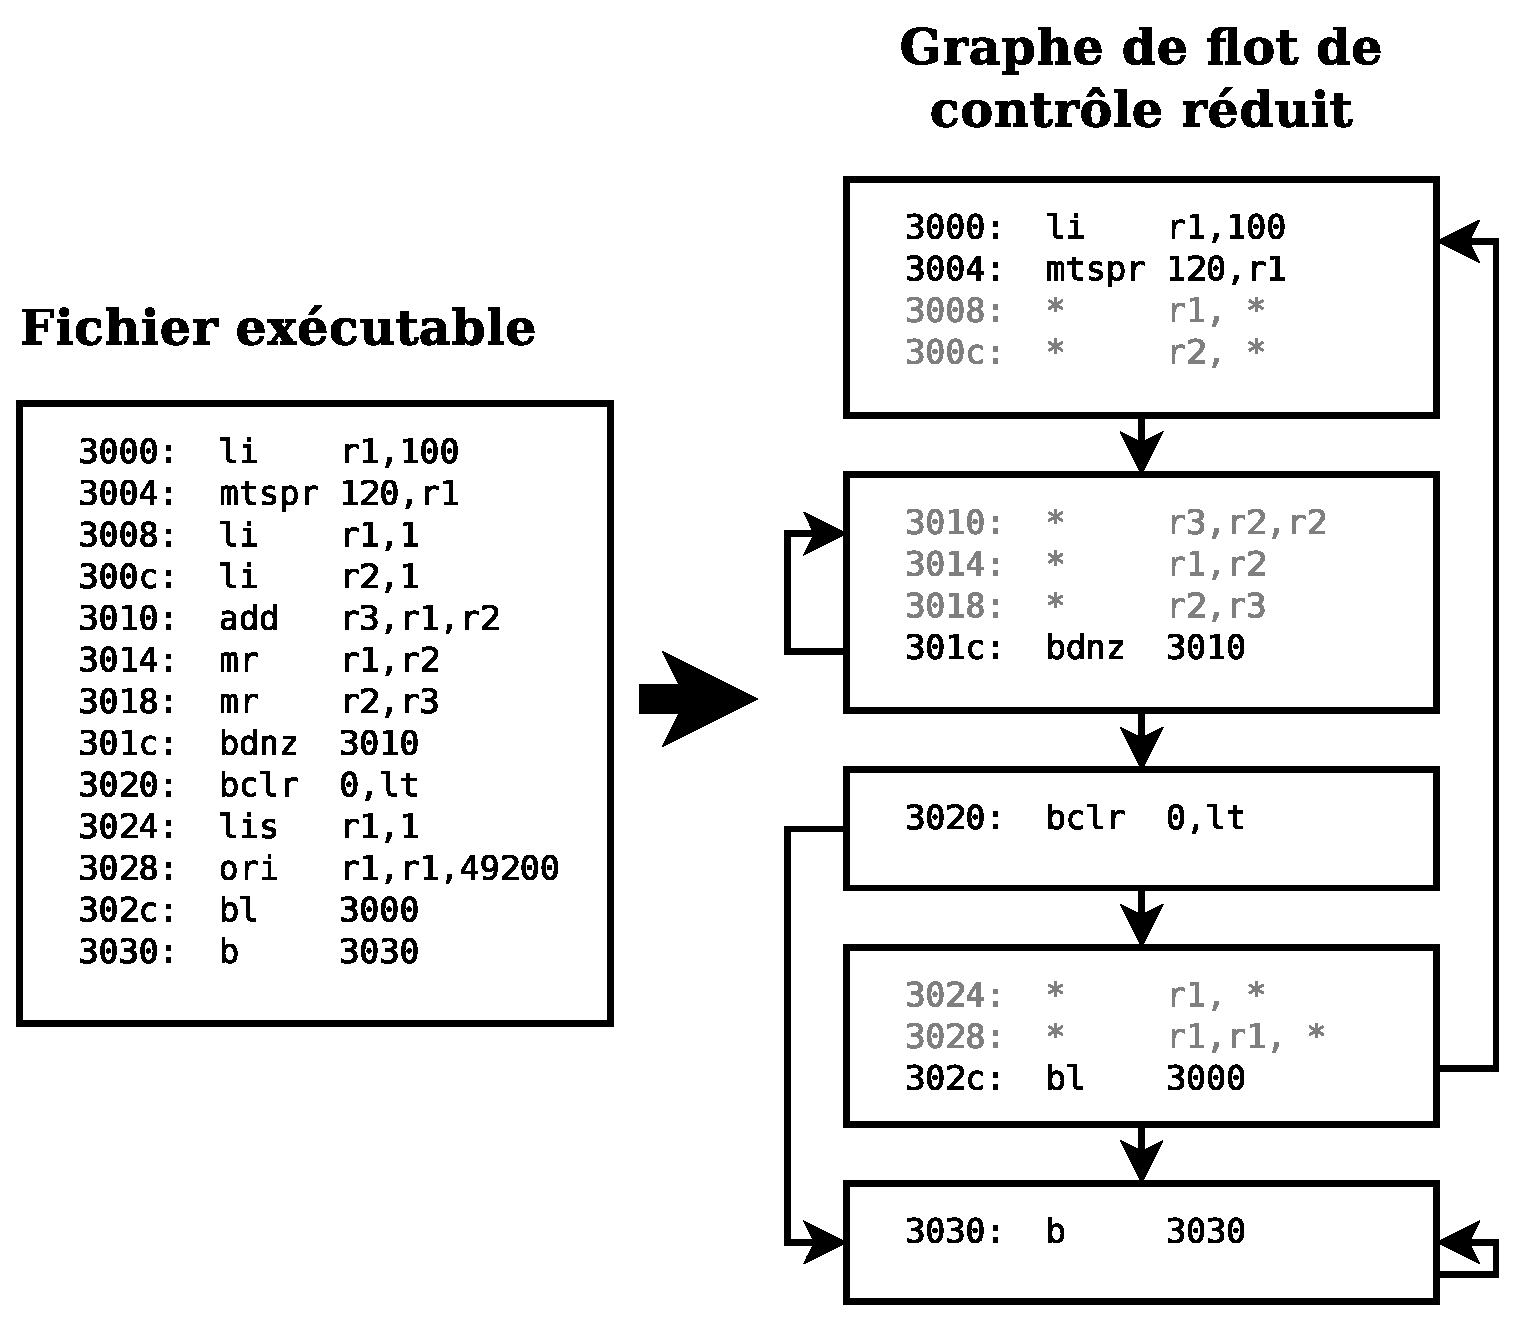
\includegraphics[scale=.3]{cfg.eps}
      \caption{Exemple schématique}
    \end{figure}
  \end{frame}

  % Futur concerant le second point
  \section{Perspectives}
  \begin{frame}
    \frametitle{\secname}

    \begin{itemize}
      \item Poursuite du travail sur l'outil
      \item Production d'un modèle du matériel multi-c{\oe}ur
      \item Spécialisation de l'algorithme d'exploration de l'espace d'état
    \end{itemize}
  \end{frame}
\end{document}
